\documentclass[pdf,table]{beamer}
\usepackage{graphicx,hyperref,pdfpages}
\usepackage{tikz}
\usepackage{textpos}
\usepackage{longtable}
\usepackage{listings}
\usepackage{color}
\usetikzlibrary{arrows}
\usetikzlibrary{positioning,chains,fit,shapes,calc}
\usetikzlibrary{mindmap}
\usetikzlibrary{shapes.multipart}
%\usepackage[table]{xcolor}
%\usepackage{booktabs}
\usepackage[style=numeric,backend=biber]{biblatex}
\addbibresource{../CST4025.bib}
\setbeamertemplate{bibliography item}{\insertbiblabel}

%
%defin colours
\definecolor{codegreen}{rgb}{0,0.6,0}
\definecolor{codegray}{rgb}{0.5,0.5,0.5}
\definecolor{codepurple}{rgb}{0.58,0,0.82}
\definecolor{backcolour}{rgb}{0.95,0.95,0.92}
\definecolor{delim}{rgb}{20,105,176}



\lstdefinelanguage{CTO}{
	keywords={abstract, asset, by, concept, default, enum, event, identified, Integer, o, participant, String, transaction },
	comment=[l]{//},
	comment=[s]{/*}{*/},
	string=[b]",
	sensitive=true,
}

\lstdefinelanguage{ACL}{
	keywords={transaction,condition,rule,description,participant,operation,resource,action,ALLOW,READ,ALL,CREATE,UPDATE,DELETE,ANY,DENY},
	comment=[l]{//},
	comment=[s]{/*}{*/},
	string=[b]",
	sensitive=true,
}

%define Javascript language
\lstdefinelanguage{JavaScript}{
keywords={typeof, new, true, false, catch, function, return, null, catch, switch, var, if, in, while, do, else, case, break},
keywordstyle=\color{blue}\bfseries,
ndkeywords={class, export, boolean, throw, implements, import, this},
ndkeywordstyle=\color{darkgray}\bfseries,
identifierstyle=\color{black},
sensitive=false,
comment=[l]{//},
morecomment=[s]{/*}{*/},
commentstyle=\color{purple}\ttfamily,
stringstyle=\color{red}\ttfamily,
morestring=[b]',
morestring=[b]"
}
%define json language
\colorlet{punct}{red!60!black}
\definecolor{background}{HTML}{EEEEEE}
\definecolor{delimiter}{RGB}{20,105,176}
\colorlet{numb}{magenta!60!black}

\lstdefinelanguage{json}{
    numbers=left,
    numberstyle=\scriptsize,
    stepnumber=1,
    numbersep=8pt,
    showstringspaces=false,
    breaklines=true,
    frame=lines,
    backgroundcolor=\color{background},
    literate=
     *{0}{{{\color{numb}0}}}{1}
      {1}{{{\color{numb}1}}}{1}
      {2}{{{\color{numb}2}}}{1}
      {3}{{{\color{numb}3}}}{1}
      {4}{{{\color{numb}4}}}{1}
      {5}{{{\color{numb}5}}}{1}
      {6}{{{\color{numb}6}}}{1}
      {7}{{{\color{numb}7}}}{1}
      {8}{{{\color{numb}8}}}{1}
      {9}{{{\color{numb}9}}}{1}
      {:}{{{\color{punct}{:}}}}{1}
      {,}{{{\color{punct}{,}}}}{1}
      {\{}{{{\color{delimiter}{\{}}}}{1}
      {\}}{{{\color{delimiter}{\}}}}}{1}
      {[}{{{\color{delimiter}{[}}}}{1}
      {]}{{{\color{delimiter}{]}}}}{1},
}
%\lstdefinelanguage{json}{
%    numbers=left,
%    numberstyle=\scriptsize,
%    stepnumber=1,
%    numbersep=8pt,
%    showstringspaces=false,
%    breaklines=true,
%    frame=lines,
%    backgroundcolor=\color{backcolour},
%    literate=
%     *{\{}{{{\color{delim}{\{}}}}{1}
%      {\}}{{{\color{delim}{\}}}}}{1}
%      {[}{{{\color{delim}{[}}}}{1}
%      {]}{{{\color{delim}{]}}}}{1},
%}



\lstdefinestyle{mys}{
	backgroundcolor=\color{backcolour},
	commentstyle=\color{codegreen},
	keywordstyle=\color{magenta},
	stringstyle=\color{codepurple},
	numberstyle=\color{codegray},
	basicstyle=\ttfamily\tiny,
	breakatwhitespace=false,
	breaklines=true
	captionpos=b,
	keepspaces=true,
	numbers=left,
	numbersep=5pt,
	showspaces=false,
	showstringspaces=false,
	showtabs=false,
	tabsize=2}
\lstset{style=mys}



\tikzset{every matrix/.style={ampersand replacement=\&,column sep=1.75cm,row sep=2cm},
		BTWMat/.style={ampersand replacement=\&, column sep=0.75cm,row sep=1cm},
		eulerMat/.style={ampersand replacement=\&,column sep=1.1cm,row sep=2cm},
		vertexHighlight/.style={circle,fill=red!80,inner sep=.1cm,text=white},
		vertex/.style={circle,fill=blue!80,inner sep=.1cm,text=white},
		bank/.style={rectangle,fill=blue!50,inner sep=0.1cm,text=black!80}
		edge/.style={--,line width=2pt},
		Dedge/.style={->,line width=2pt},
		DedgeT/.style={->,line width=1pt},
		BiEdge/.style={<->,line width=2pt},
		BiEdgeT/.style={BiEdge,line width=1pt},
		edgeHighlight/.style={--,line width=2pt,color=red},
		loop/.style={min distance=10mm, line width=2pt},
		loopT/.style={min distance=-10mm, line width=1pt},
		label/.style = { rectangle, rounded corners, draw,
		                 minimum width = 2em, fill = yellow!50,
		                 text = red, font = \tiny\bfseries },
		labelT/.style = { circle, draw, line width=1pt,
		                 minimum width = 1em, fill = yellow!50,
		                 text = red, font = \tiny\bfseries },
		every node/.style={align=center}}



\newcommand{\cwideadline}{3$^{rd}$ November 2019}
\newcommand{\cwiideadline}{5$^{th}$ January 2020}
%\newcommand{\cwiiideadline}{31$^{st}$ March 2017}
%\newcommand{\cwiiideadline}{15$^{th}$ April 2018}
\newcommand{\resitdeadline}{1$^{st}$ August 2020}
\newcommand{\deferraldeadline}{1$^{st}$ August 2020}
\newcommand{\deferraldeadlineMay}{1$^{st}$ May 2020}
\newcommand{\moduleCode}{CST4025}
\newcommand{\moduleLeader}{Dr Ian Mitchell }
\newcommand{\theauthor}{Dr Ian Mitchell }
\newcommand{\academicyear}{2019-20}
\newcommand{\email}{i.mitchell@mdx.ac.uk}
\newcommand{\moduleTitle}{Blockchain Development}
\newcommand{\office}{T108}
\newcommand{\officehours}{Autumn \& Winter Terms: Tuesdays 1515-1615hrs; and, Wednesdays 1415-1515hrs}
\newcommand{\tel}{0208-411-6014}
\newcommand{\deptName}{Computer Science}
%\newcommand{\officehours}{Friday 1100\--1300hrs Autumn Term \\ Thursday 1400\--1600hrs Winter Term}
%\newcommand{\officehours}{Autumn Term: Mondays 1300\--1500hrs \\ Winter Term: Thursdays 1400\--1600hrs

\def\bitcoinA{%
  \leavevmode
  \vtop{\offinterlineskip %\bfseries
    \setbox0=\hbox{B}%
    \setbox2=\hbox to\wd0{\hfil\hskip-.03em
    \vrule height .3ex width .15ex\hskip .08em
    \vrule height .3ex width .15ex\hfil}
    \vbox{\copy2\box0}\box2}}




\mode<presentation>{
\usetheme{Madrid}
\usecolortheme{beaver}
}

\newcommand{\theweek}{2}
\renewcommand{\theequation}{\theweek.\arabic{equation}}

\title[\moduleCode:L\theweek]{\moduleTitle \\ Week: \theweek \\ Title: Data Modelling} 

%[\includegraphics[scale=0.2]{../logo/mdxSmall}]
\institute[]{\includegraphics[scale=0.25]{../../../logo/mdxSmall} \\ Middlesex University, \\Dept. of Computer Science, \\London}
\author[\email]{\moduleLeader}
\date{\today}




\begin{document}
	\begin{frame}
		\titlepage
	\end{frame}


\addtobeamertemplate{frametitle}{}{%
\begin{textblock*}{100mm}(.94\textwidth,-0.85cm)
\includegraphics[scale=0.1]{../../../logo/transparent}
\end{textblock*}}

	\begin{frame}{Lecture }
		\begin{block}{Aims}
			Essentially, there are three steps for blockchain development, which we will learn over the coming weeks. The first step is Data Modelling, using CTO.
		\end{block}
	\end{frame}

	\begin{frame}{Lecture Objectives}
		\begin{block}{Knowledge}
			\begin{itemize}
				\item Differentiate between Assets, Participants, Transactions and Events
				\item Model and develop blockchain code to implement a data structure
				\item Background and context of Hyperledger frameworks
				\item See how blockchain can be applied by looking at use cases.
			\end{itemize}	
			{\bf Skills}
			\begin{itemize}
				\item Implement and develop the data model for a blockchain using ConcerTO (CTO).
			\end{itemize}
		\end{block}
	\end{frame}

\begin{frame}{Hyperledger}
	\begin{columns}[T]
		\begin{column}{0.40\textwidth}
		{\bf Open Source}
			\begin{itemize}
				\item Free
				\item Distribute
				\item Copy
				\item Edit and Modify
				\item License
			\end{itemize}
		\end{column}
		\begin{column}{0.58\textwidth}
			{\bf Open Governance}
			\begin{itemize}
				\item Transparent in decisions
				\item Development processes
				\item Maintainers
				\item Community
				\item The Steering Committee (TSC)
				\item See how blockchain can be applied by looking at use cases.
				\item Active contributors are eligible to participate
				\item Bring your nominations
				\item Cast your vote
				\item Not just a piece of code, its a movement
			\end{itemize}
		\end{column}
	\end{columns}	
\end{frame}

\begin{frame}{Hyperledger Structure}
	\begin{tikzpicture}[scale=0.5, line width=2pt]
%		\node at (1,9) [sqrVertex] (1){Model .cto \nodepart{two}Assets \\Participants\\ Transactions};	
%		\node at (4,9) [sqrVertex] (2){Script .js \nodepart{two} Transaction \\Functions\\};
%		\node at (7,9) [sqrVertex] (3){Access .acl \nodepart{two} Access \\ Control \\ Rules};
%		\node at (10,9) [sqrVertex] (4){Query .qry \nodepart{two} Query \\ Definitions\\};
%		
	        \node  [sqrVertex] (1){Model .cto \nodepart{two}Assets \\Participants\\ Transactions};	
		\node  [sqrVertex] (2) [right=of 1] {Script .js \nodepart{two} Transaction \\Functions\\};
		\node  [sqrVertex] (3) [right=of 2] {Access .acl \nodepart{two} Access \\ Control \\ Rules};
		\node  [sqrVertex] (4) [right=of 3] {Query .qry \nodepart{two} Query \\ Definitions\\};
	
%		\node at (1,6) [zero] (5){};
%		\node at (4,6) [zero] (6){};
%		\node at (7,6) [zero] (7){};
%		\node at (10,6) [zero] (8){};
		\node [zero] (5)[below=of 1]{};
		\node [zero] (6)[below=of 2]{};
		\node [zero] (7)[below=of 3]{};
		\node [zero] (8)[below=of 4]{};
		\node [zero] (9)[right=of 6]{};
%		\draw[blue!80] (5) -- (8);
		\draw[blue!80] (1) -- (5);
		\draw[blue!80] (2) -- (6);
		\draw[blue!80] (3) -- (7);
%		\draw[blue!80] (4) -- (8);

		\draw[blue!80] (1.south) --  (5.south) -- (8.west)--(4.south);
		
%		\node [sqrVertex] (10) [right below=of 6] {.bna \nodepart{two} Business \\ Network \\ Archive};
		\node [sqrVertex] (10) [below=of 9] {.bna \nodepart{two} Business \\ Network  \\Archive};
		\draw[blue!80] (9) -- (10);

		\node [zero] (20) [below right=of 10] {};
		\node [zero] (21) [below left=of 10] {};
		\node [zero] (22) [below=of 10]{};
		\node [sqrVertex] (11) [below =of 20] {Hyperledger Fabric\nodepart{two}Cloud\\Local};
		\node [sqrVertex] (12) [below =of 21] {Web Browser \nodepart{two} Node.js\\Online};
		\draw[blue!80] (10) 	-- (22);
		\draw[blue!80] (12.north) -- (21.west) -- (22.north) --(20.east)-- (11.north);
	\end{tikzpicture}
\end{frame}


%hyperledger architecture paper 1
\begin{frame}{Hyperledger Architecture \cite{hyperledger:1}}
\begin{itemize}
	\item Consensus 
	\item Smart Contract 
	\item Communication
	\item Data Store
	\item Cryptography
	\item Policy
	\item Identity
	\item API
	\item Interoperation
\end{itemize}
\end{frame}

\begin{frame}{Hyperledger Architecture \cite{hyperledger:1}}
	{\bf Consensus}
\begin{itemize}
	\item Verify the correctness of the set of transactions
	\item A block is composed of multiple transactions
	\item Concur with other nodes
	\item Which of these can be trusted?
	\item Also provides some ordering.
	\item Consensus algorithm:
		\begin{itemize} \pause
			\item Confirms the correctness of transactions in a block, according to the consensus algorithms deployed and the policies applied.
			\item Once the block is confirmed, then it enters the blockchain, so consensus algorithm has to agree on order the blocks are added
			\item Interact and complete smart contract layer 
		\end{itemize}
\end{itemize}
\end{frame}

\begin{frame}{Supply Chain Management}
	\begin{columns}[T]
		\begin{column}{0.48\textwidth}
			\begin{itemize}
				\item XXX 
			\end{itemize}
		\end{column}
		\begin{column}{0.48\textwidth}
			{\bf XXX}
		\end{column}
	\end{columns}	
\end{frame}


\begin{frame}{Provenance}
	\begin{columns}[T]
		\begin{column}{0.48\textwidth}
			\begin{itemize}
				\item XXX 
			\end{itemize}
		\end{column}
		\begin{column}{0.48\textwidth}
			{\bf XXX}
		\end{column}
	\end{columns}	
\end{frame}

\begin{frame}{Property}
	\begin{columns}[T]
		\begin{column}{0.48\textwidth}
			\begin{itemize}
				\item XXX 
			\end{itemize}
		\end{column}
		\begin{column}{0.48\textwidth}
			{\bf XXX}
		\end{column}
	\end{columns}	
\end{frame}

\begin{frame}{Finance}
	\begin{columns}[T]
		\begin{column}{0.48\textwidth}
			\begin{itemize}
				\item XXX 
			\end{itemize}
		\end{column}
		\begin{column}{0.48\textwidth}
			{\bf XXX}
		\end{column}
	\end{columns}	
\end{frame}


\begin{frame}{Do I need a blockchain?}{adapted from EdX.org}
	\begin{itemize} %alter this and adapt
           \item There is a need for a shared common database
           \item The parties involved with the process have conflicting incentives, or do not have trust among participants
           \item There are multiple parties involved or writers to a database
           \item There are currently trusted third parties involved in the process that facilitate interactions between multiple parties who must trust the third party. This could include escrow services, data feed providers, licensing authorities, or a notary public
           \item Cryptography is currently being used or should be used. Cryptography facilitates data confidentiality, data integrity, authentication, and non-repudiation
           \item Data for a business process is being entered into many different databases along the lifecycle of the process. It is important that this data is consistent across all entities, and/or digitization of such a process is desired
           \item There are uniform rules governing participants in the system
           \item Decision making of the parties is transparent, rather than confidential
           \item There is a need for an objective, immutable history or log of facts for parties’ reference
           \item Transaction frequency does not exceed 10,000 transactions per second.
	\end{itemize}
\end{frame}



\begin{frame}{When not to use Blockchain}{adapted from EdX.org}
	\begin{itemize}
           \item The process involves confidential data
           \item The process stores a lot of static data, or the data is quite large
           \item Rules of transactions change frequently
           \item The use of external services to gather/store data.
	\end{itemize}
\end{frame}


\begin{frame}{Flowchart}{Do I need a blockchain flowchart}
	{\bf Adapted from EdX.org and \cite{yaga2018blockchain}}
\begin{tikzpicture}
	\node	at (0,8) [rectVertex]	(0){Shared consistent data};
	\node	at (2,8) [rectVertex] (2){Shared entity generation};
	\node 	at (4,8) [rectVertex] (4){Confliction or Trust};
	\node 	at (6,8) [rectVertex] (6){Participants rules are uniform};
	\node  	at (8,8) [rectVertex] (8){Immutable?};
	\node 	at (10,8)[rectVertex] (10){Public};
	
	\node 	[zero,below=of 0] (1){};
	\node	[zero, below=of 2] (3){};
	\node	[zero, below=of 4] (5){};
	\node 	[zero, below=of 6] (7){};
	\node 	[zero, below=of 8] (9){};
	\node 	[zero, below=of 10] (11){};

	\node [rectVertex, below=of 9](12){Permissionless};
	\node [rectVertex, below=of 11](13){Permissioned};
	\node [rectVertex, below=of 5](14){Blockchain not required};
	\draw (0) -- (1);
	\draw (2) -- (3);
	\draw (4) -- (5);
	\draw (6) -- (7);
	\draw (8) -- (9);
	\draw (10) -- (11);
	\draw (1)--(9);
	\draw (5)--(14);	
	\draw (11) -- node[left ]{Yes} (12.north);
	\draw (11) -- node[right ]{No} (13);
	
	
\end{tikzpicture}
\end{frame}

\begin{frame}{Participants}
	\begin{columns}[T]
		\begin{column}{0.48\textwidth}
			%explain participants are users that interact with various levels of access and privileges in a business network
			{\bf Individual}
			\begin{itemize}
				\item User 
				\item end-users 
				\item more individuals than businesses 
			\end{itemize}
			{\bf Organisational}
			\begin{itemize}
				\item service providers
				\item manufacturers
				\item an organisation can exist independent of the individuals %contentious, but no one is irreplaceable
				\item Expansion during growth
				\item Reduction during downturn
		\end{itemize}
		\end{column}
		\begin{column}{0.48\textwidth}
			\begin{itemize}
				\item Individuals are members of an organisation and act on behalf of the organisation, and with authority of that organisation.
			\end{itemize}			
			{\bf System or Device}
			\begin{itemize}
				\item special kind of individual
				\item How many systems does Middlesex have? %(misis, arc, timetabling, mylearning, kortext, email, .....)
				\item Systems belong to organisation
				\item Systems act on behalf of organisation
				\item Autonomous devices 
				\item Possibility of more autonomous agents in the future
			\end{itemize}
		\end{column}
	\end{columns}	
\end{frame}


\begin{frame}{Assets}
	\begin{columns}[T]
		\begin{column}{0.48\textwidth}
			\begin{itemize}
				\item exchanges of information between participants
				\item participants have a degree of autonomy
				\item assets are quite passive
				\item assets have meaning to participants
				\item assets have value
				\item therefore represent the value exchanged between participants

			\end{itemize}
		\end{column}
		\begin{column}{0.48\textwidth}
			\begin{itemize}
				\item Tangible: cars, products, goods
				\item Intangible: staff morale, IP, policies, data, knowledge, information
				\item Literally? Everything on blockchain is intangible, its digital.
				\item Intangible assets on blockchain, do have value, it is just not explicit

			\end{itemize}
		\end{column}
	\end{columns}	
\end{frame}


\begin{frame}{Asset Structure}
	\begin{columns}[T]
		\begin{column}{0.48\textwidth}
			\begin{itemize}
				\item Attributes: Properties and Relationships 
				\item Properties: characteristics of an object, manufacturer, model, registration, car.
				\item Asset Type
				\item Asset Instance
			\end{itemize}
		\end{column}
		\begin{column}{0.48\textwidth}
			\begin{itemize}
				\item Relationships: reference to another asset
				\item car: has insurance, owner, mot, tax
				\item Modelling the Assets, participants and relationships
				\item Gneral rule of thumb: reduce big assets into smaller assets with relationships
				\item Separation of concerns
				\item domain-specific - colour is an asset of a car? %to a paint manufacture colour is the asset, to a car manufacturer colour is an attribute
			\end{itemize}
		\end{column}
	\end{columns}	
\end{frame}



\begin{frame}{Ownership \& Lifecycles}
	\begin{columns}[T]
		\begin{column}{0.48\textwidth}
			\begin{itemize}
				\item associative relationship %we associate x with y
				\item does a person own a car?
				\item is car an attribute of person?
				\item It is a mapping between participant (individual) and the car
				\item ownership is a concept
				\item blockchains are often used to record ownership and changes in ownership
			\end{itemize}
		\end{column}
		\begin{column}{0.48\textwidth}
			\begin{itemize}
				\item Provenance
				\item properties of asset modified
				\item asset ceases to exist
				\item Bank loan
				\item Transformation involves: division and aggregation
				\item Transformation type: homogenous and heterogenous
			\end{itemize}
		\end{column}
	\end{columns}	
\end{frame}

% chapter 6 in Naur
\begin{frame}{Asset Life Cycles}
	\begin{columns}[T]
		\begin{column}{0.48\textwidth}
			{\bf Division \& Homogeneous  }
			\begin{itemize}
				\item Reduction of large asset
				\item Leather 
				\item Divide leather up for manufacturers
				\item  Leather comes from the same animal 
				\item  Just divided up into smaller pieces
				\item It is the same and undergone a homogeneous transformation
			\end{itemize}
		\end{column}
		\begin{column}{0.48\textwidth}
			{\bf Aggregate \& Heterogeneous}
			\begin{itemize}
				\item transform the leather into a shoe 
				\item leather has been combined with other material
				\item leather has been aggregated to form a shoe
				\item components have undergone a heterogeneous transformation
				\item Tangible
				\item Intangible? %mergers or acquisitions
			\end{itemize}
		\end{column}
	\end{columns}	
\end{frame}

\begin{frame}{Participants, Assets and Transactions}
	\begin{columns}[T]
		\begin{column}{0.48\textwidth}
			\begin{itemize}
				\item Assets evolve via transactions
				\item Insurance policy % requested, refined, signed, agreed, delivered, paid (installments), claimed-against, paid-out against, invalidated, renewed, premium recalculation, etc..
				\item Participants evolve via transactions
				\item Difference: form v. function
				\item Both are resources % birds, insects and bats fly - they are not related
			\end{itemize}
		\end{column}
		\begin{column}{0.48\textwidth}
			\begin{itemize}
				\item Related in the most general sense
				\item Because they both have lifecycles described by transactions does not make them equal
				\item Participants: Users
				\item Assets: tangible or intangible
			\end{itemize}
		\end{column}
	\end{columns}	
\end{frame}

\begin{frame}{Exchange}
	\begin{columns}[T]
		\begin{column}{0.48\textwidth}
			\begin{itemize}
				\item Record change
				\item Change is captured via a transaction
				\item buyer pays owner in exchange of possesion of asset
				\item Lucy pays \pounds 289 for a printer on 28th March 2019
				\item Generalise and particular (instance)

			\end{itemize}
		\end{column}
		\begin{column}{0.48\textwidth}
			\begin{itemize}
				\item Generalisation describes semantics of transaction
				\item Particular transactions describes an instance
				\item Lucy received a receipt for her transaction
				\item The receipt is a copy of the transaction
				\item The computer shop also keeps a record of the receipt
				\item It the printer breaks after 2 days, we get to find out the true nature of the transaction
				\item otherwise the transaction is implicit
				\item you buy, you own
			\end{itemize}
		\end{column}
	\end{columns}	
\end{frame}


\begin{frame}{Low-consequence transactions}
	\begin{columns}[T]
		\begin{column}{0.48\textwidth}
			\begin{itemize}
				\item implicitness has downsides % no
				\item trust
				\item laws on fair transactions
				\item Sale of Goods Act
				\item Lack of explicit contract, simplifies the transaction
				\item Receipt
			\end{itemize}
		\end{column}
		\begin{column}{0.48\textwidth}
			\begin{itemize}
				\item reducing friction
				\item 
			\end{itemize}
		\end{column}
	\end{columns}	
\end{frame}



\begin{frame}{Case Study}
	\begin{columns}[T]
		\begin{column}{0.48\textwidth}
			{\bf Letter of Credit (L/C)}
			\begin{itemize}
				\item How was trade possible?
				\item Unsafe to travel with valuables?
				\item Go back 500 years
				\item Bank writes L/C.
				\item L/C is used to exchange goods.
			\end{itemize}
		\end{column}
		\begin{column}{0.48\textwidth}
			{\bf Example}
			\begin{itemize}
				\item Company Argo banks with Bank of Portugal 
				\item Company Argo is based in Lisbon 
				\item Company Baa is based in London
				\item Company Baa banks with Bank of England
				\item Company Baa sells Wool
				\item Company Argo wants to buy some Wool from Company Baa 
			\end{itemize}
		\end{column}
	\end{columns}	
\end{frame}



\begin{frame}{Case Study - Scenario}
	\begin{columns}[T]
		\begin{column}{0.48\textwidth}
			\begin{itemize}
				\item Argo gets L/C from Bank of Portugal 
				\item Argo representative travels to London 
				\item Agrees on price and quantity
				\item Pays for goods with L/C
				\item L/C is honoured by Bank of England
				\item Bank of England pay Baa
				\item Bank of Portugal pay Bank of England
			\end{itemize}
		\end{column}
		\begin{column}{0.48\textwidth}
			{\bf What can go wrong?}
			\begin{itemize}
				\item Trust?
				\item It takes 1 months to transport Goods from London to Lisbon 
				\item Goods could arrive in bad condition
				\item Goods may not arrive
				\item Goods could be destroyed in transit
				\item Value of goods could depreciate during journey
				\item Export license is denied
			\end{itemize}
		\end{column}
	\end{columns}	
\end{frame}

\begin{frame}{London \--- Lisbon}
	\begin{columns}[T]
		\begin{column}{0.48\textwidth}
			\begin{itemize}
				\item Line of credit needs some further details?
			\end{itemize}
		\end{column}
		\begin{column}{0.48\textwidth}
			\begin{block}{Letter of Credit (L/C)}
				Bank of Portugal hereby issues the amount of 400 Escudos payable immediately. In accordance with L/C 48722.
				
			\end{block}
		\end{column}
	\end{columns}	
\end{frame}

\begin{frame}{London \---Lisbon}
	\begin{columns}[T]
		\begin{column}{0.48\textwidth}
			\begin{itemize}
				\item Line of credit needs some further details?
				\item What is for?
				\item Invoice?
				\item Proof of delivery
				\item Insurance of goods during transit
				\item Pay half now, and half on delivery
				\item Charges for L/C
			\end{itemize}
		\end{column}
		\begin{column}{0.48\textwidth}
			\begin{block}{Letter of Credit (L/C)}
				Bank of Portugal hereby issues the amount of 400  Escudos payable immediately. In accordance with L/C 48722. This L/C should be accompanied with:
				\begin{enumerate}
					\item Bill of Lading (B/L)
					\item Packing List
					\item Invoice
				\end{enumerate}
				
			\end{block}
		\end{column}
	\end{columns}	
\end{frame}

\begin{frame}{London\---Lisbon}
	\begin{columns}[T]
		\begin{column}{0.48\textwidth}
			\begin{itemize}
				\item Bill of Lading
				\item Ensure goods are present and correct
				\item Ensure goods are in order
				\item Weight, Condition and Quality.
			\end{itemize}
		\end{column}
		\begin{column}{0.48\textwidth}
			\begin{block}{Bill of Lading (B/L)}
				\begin{itemize}
					\item Shipper: Baa
					\item Consignee: Argo
					\item 1 Ton of Wool
					\item London to Lisbon 
					\item Frieght Charges: 50 Escudos 
				\end{itemize}
			\end{block}
		\end{column}
	\end{columns}	
\end{frame}

\begin{frame}{London\---Lisbon}
	\begin{columns}[T]
		\begin{column}{0.48\textwidth}
			\begin{itemize}
				\item Export License
				\item Allowing the export of goods
				\item Import License 
				\item Allowing the import of goods
			\end{itemize}
		\end{column}
		\begin{column}{0.48\textwidth}
			\begin{block}{Export}
				On 20th March 1784 UK Govt permit the export of 1 ton: Wool. Consignment: 32496. Company: Baa.
			\end{block}
			\begin{block}{Import}
				On 20th March 1784 Potuguese Govt permit the import of 1 ton: Wool. Tax Levy: 10 Escudos. Consignment: 10473. Company: Argo. 
			\end{block}
		\end{column}
	\end{columns}	
\end{frame}

\begin{frame}{London\---Lisbon}
	\begin{itemize}
		\item Bank of Portugal
		\item Bank of England
		\item Meeting, whereby Portugal would honour their L/C and pay Bank of England.
		\item Trust
		\item Bank of England trusts Bank of Portugal
		\item Charges made to Argo
	\end{itemize}
\end{frame}

\begin{frame}{Case Study}
	\begin{columns}[T]
		\begin{column}{0.48\textwidth}
			\begin{enumerate}
				\item Argo requests goods from Baa in exchange for money
				\item Baa accept the trade deal
				\item Argo asks BoP for a L/C in favor of the Baa 
				\item BoP supplies a L/C in favour of Baa, and payable to BoE  
				\item BoE accepts the L/C on behalf of Baa
				\item Baa applies for an E/L
			\end{enumerate}
		\end{column}
	\begin{column}{0.48\textwidth}
		\begin{enumerate}
			\setcounter{enumi}{6}
			\item E/L is granted
			\item Baa prepares shipment
			\item Logistics company validate E/L and supplies a B/L to Baa
			\item BoE claims half the payment from the BoP
			\item BoP transfers half the payment to BoE
			\item Logistics ships goods to location
			\item BoP pays remain amount to BoE
		\end{enumerate}
	\end{column}
	\end{columns}	
\end{frame}

\begin{frame}{Case Study}
       	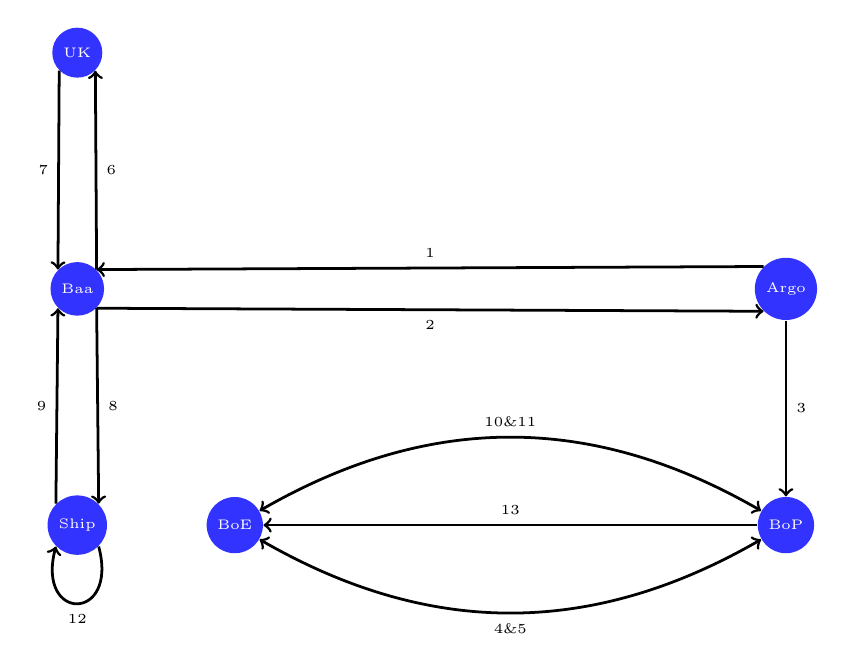
\begin{tikzpicture}[scale=1.0,font=\tiny]
       		\node at (9,9) [vertex] (1){Argo};
       		\node at (0,9) [vertex]	(2){Baa};
       		\node at (0,6) [vertex] (3){Ship};
       		\node at (0,12) [vertex] (4){UK};
       		\node at (2,6) [vertex] (5){BoE};
       		\node at (9,6) [vertex] (6){BoP};
		%zero nodes
		

       		\draw (1.north west) edge[DedgeT] node[above]{1}  (2.north east);
       		\draw (2.south east) edge[DedgeT] node[below]{2}  (1.south west);
		\draw (2.north east) edge[DedgeT] node[right]{6}  (4.south east);
		\draw (4.south west) edge[DedgeT] node[left]{7}  (2.north west);
		\draw (2.south east) edge[DedgeT] node[right]{8}  (3.north east);
		\draw (3.north west) edge[DedgeT] node[left]{9}  (2.south west);
		\draw (1) edge[DedgeT] node[right]{3} (6);
		\draw (5) edge[BiEdgeT, bend right] node[below]{4\&5} (6);
		\draw (5) edge[BiEdgeT, bend left] node[above]{10\&11} (6);
		\draw (6) edge[DedgeT] node[above]{13} (5);
		\draw (3.south east) edge[->,loop below, line width=1pt] node[below]{12} (3.south west);
       	\end{tikzpicture}
\end{frame}

\begin{frame}{Case Study - Assets \& Paricipants}
	\begin{columns}[T]
		\begin{column}{0.48\textwidth}
			{\bf Data}
			\begin{itemize}
				\item transactions
				\item Letter of Credit
				\item Bill of Lading
				\item Export License
				\item trade agreement
				\item Payment
				\item Shipment
			\end{itemize}
		\end{column}
		\begin{column}{0.48\textwidth}
			{\bf Participants}
			\begin{itemize}
				\item Baa
				\item Argos
				\item UK govt
				\item BoE
				\item BoP
			\end{itemize}
		\end{column}
	\end{columns}	
\end{frame}

\begin{frame}{Case Study - Access}
	\begin{columns}[T]
		\begin{column}{0.48\textwidth}
			\begin{itemize}
				\item Only Argos may apply for L/C
				\item Only BoP may supply L/C
				\item Only BoE may accept L/C
				\item 
			\end{itemize}
		\end{column}
		\begin{column}{0.48\textwidth}
			{\bf XXX}
		\end{column}
	\end{columns}	
\end{frame}

\begin{frame}{Case Study - Access Generalisation}
	\begin{columns}[T]
		\begin{column}{0.48\textwidth}
			\begin{itemize}
				\item Only an importer may apply for L/C; 
				\item Only an importer's bank may supply an L/C;
				\item Only an exporter's bank may accept an L/C;
				\item Only an exporter may requests an E/L
				\item Only a regulatory authority may supply an E/L;
				\item Only an exporter may prepare shipment;
		\end{itemize}
		\end{column}
		\begin{column}{0.48\textwidth}
			\begin{itemize}
				\item Only a logistics company may supply a B/L;
				\item Only a carrier may update a shipment location;
				\item Only an importer's bank may send money; and, 
				\item only an exporter's bank may receive money
			\end{itemize}
		\end{column}
	\end{columns}	
\end{frame}



\begin{frame}{Case Study}
	\begin{columns}[T]
		\begin{column}{0.48\textwidth}
			{\bf Friction}
			\begin{itemize}
				\item  line of credit
				\item export licenses
				\item agreements
				\item bill of lading
				\item overheads
				\item Speed, but friction remains
			\end{itemize}
		\end{column}
		\begin{column}{0.48\textwidth}
			{\bf Frictionless?}
			\begin{itemize}
				\item payment linked to documentary completion
				\item payment linked to progress of shipment?
				\item trade agreement on a single blockchain
				\item implement a smart contract
			\end{itemize}
		\end{column}
	\end{columns}	
\end{frame}

\begin{frame}{Case Study - Benefits}
	\begin{itemize}
		\item through [dis]trust and [dis]honesty came the inspiration for L/C and B/L;
		\item applying for E/L, L/C and B/L is an overhead and increases turn-around-times;
		\item Automation has reduced this, but not changed it much.
		\item What are the benefits of blockchain?
	\end{itemize}
\end{frame}

\begin{frame}{Case Study - Benefits}
	\begin{itemize}
		\item conditional installments 
		\item (dis)intermediaries
		\item trust
		\item auditable
		\item secure
		\item sustainable
		\item extensible
		\item communication 
		\item increase accountability, minimise risk
	\end{itemize}
\end{frame}


%\begin{frame}{ConcerTO, CTO, Design}
%	\begin{columns}[T]
%		\begin{column}{0.48\textwidth}
%			\begin{itemize}
%				\item<1-> Enumerators
%				\item<2-> Concepts
%				\item<3-> Arrays
%				\item<4-> asset
%				\item<5-> participant
%				\item<6-> transaction
%				\item<7-> event
%				\item<8-> namespace
%				\item<9-> comments
%			\end{itemize}
%		\end{column}
%		\begin{column}{0.48\textwidth}
%			\begin{itemize}
%				\item 
%		\end{column}
%	\end{columns}	
%\end{frame}

	
\begin{frame}[fragile]{CTO}{Enumerator Types}
	\begin{columns}[T]
		\begin{column}{0.48\textwidth}
			\begin{itemize}
				\item String: UTF8
				\item Integer: 32bit signed number 
				\item Double: double precision 64bit number
				\item Long: 64bit signed number 
				\item DateTime: ISO8061 DateTime
				\item Boolean: true, false
			\end{itemize}
		\end{column}
		\begin{column}{0.48\textwidth}
			{\bf Listing}
			\begin{lstlisting}[language=CTO]
enum enumeratorName {
	o ENUM1
	o ENUM2
}
			\end{lstlisting}
			\begin{lstlisting}[language=CTO]
enum gender{
	o MALE
	o FEMALE
	o NONBINARY 
}
			\end{lstlisting}
		\end{column}
	\end{columns}	
\end{frame}

\begin{frame}[fragile]{CTO}{Concepts}
	\begin{columns}[T]
		\begin{column}{0.48\textwidth}
			\begin{itemize}
				\item Abstract classes
				\item !Participants
				\item !Assets
				\item !Transaction
				\item No instances
				\item Extended
			\end{itemize}	
		\end{column}
		\begin{column}{0.48\textwidth}
			{\bf Listing}
			\begin{lstlisting}[language=CTO]
abstract concept address {
	o String houseNumber 
	o String streetName
	o String townName
	o String county 
	o String country default="UK"
	o String postCode regex=/RegEx/
}
			\end{lstlisting}
		\end{column}
	\end{columns}	
\end{frame}
	%(GIR 0AA)|((([A-Z-[QVf]][0-9][0-9]?)|(([A-Z-[QVf]][A-Z-[IJZ]][0-9][0-9]?)|(([A-Z-[QVf]][0-9][A-HJKPSTUW])|([A-Z-[QVf]][A-Z-[IJZ]][0-9][ABEHMNPRVWfY])))) [0-9][A-Z-[CIKMOV]]{2})/
	

\begin{frame}[fragile]{CTO}{Participants}
	\begin{columns}[T]
		\begin{column}{0.48\textwidth}
			\begin{itemize}
				\item Users
				\item identified by
				\item extend
				\item Group of users 
			\end{itemize}	
		\end{column}
		\begin{column}{0.48\textwidth}
			{\bf Listing}
\begin{lstlisting}[language=CTO]
participant person identified by personID{
	o String personID regex=/[0-9]{8}/
	o String lastName
	o String firstName
	o gender Gender
	o address Address
}
			\end{lstlisting}
		\end{column}
	\end{columns}	
\end{frame}


\begin{frame}[fragile]{CTO}{Assets}
	\begin{columns}[T]
		\begin{column}{0.48\textwidth}
			\begin{itemize}
				\item Goods, Products, Services
				\item Identified by
				\item Belonging, ownership 
				\item Relationship 
					\begin{itemize}
						\item namespace
						\item type name
						\item identifier
						\item relationship to 
						\item org.example.person\#12345678
						\item unidirectional
						\item deletes do not cascade % check
					\end{itemize}
			\end{itemize}	
		\end{column}
		\begin{column}{0.48\textwidth}
			{\bf Listing}
\begin{lstlisting}[language=CTO]
asset product identified by productID{
	o String productID regex=/[0-9]{2,4}/
	o String name 
	o Integer year default=2019 range=[1980,]
	o Double weight optional
	o DateTime transferOwnership optional
	o String description 
	--> person owner
}
			\end{lstlisting}
		\end{column}
	\end{columns}	
\end{frame}


\begin{frame}[fragile]{CTO}{Arrays}
	\begin{columns}[T]
		\begin{column}{0.48\textwidth}
			\begin{itemize}
				\item Goods, Products
				\item Services 
				\item identified by
				\item notion of belonging, ownership 
				\item relationship 
			\end{itemize}	
		\end{column}
		\begin{column}{0.48\textwidth}
			{\bf Listing}
\begin{lstlisting}[language=CTO]
asset product identified by productID{
	o String productID regex=/[0-9]{2,4}/
	o String name 
	o Integer year default=2019 range=[1980,]
	o Double weight optional
	o DateTime transferOwnership optional
	o String description 
	--> person owner
	--> person[] previousOwners
}
			\end{lstlisting}
		\end{column}
	\end{columns}	
\end{frame}
	
\begin{frame}[fragile,allowframebreaks]{CTO}{Example}
	\lstinputlisting[language=CTO,lastline=25]{example.cto}
	\lstinputlisting[language=CTO,firstnumber=26,firstline=26]{example.cto}
\end{frame}


\begin{frame}[allowframebreaks]{References}
	\printbibliography
\end{frame}
	
\begin{frame}
	\frametitle{Web Resources}
	\begin{itemize}
	\item \url{http://hyperledger.org}
	\end{itemize}
\end{frame}

\end{document}


%\begin{frame}{}
%	\begin{tikzpicture}[]
%	\end{tikzpicture}
%\end{frame}


%\begin{frame}{}
%	\begin{columns}[T]
%		\begin{column}{0.48\textwidth}
%		\end{column}
%		\begin{column}{0.48\textwidth}
%			{\bf XXX}
%%			\begin{lstlisting}
%			\end{lstlisting}
%		\end{column}
%	\end{columns}	
%\end{frame}
%
%

%\begin{frame}{X}
%	\begin{columns}[T]
%		\begin{column}{0.48\textwidth}
%			\begin{itemize}
%				\item XXX 
%			\end{itemize}
%		\end{column}
%		\begin{column}{0.48\textwidth}
%			{\bf XXX}
%		\end{column}
%	\end{columns}	
%\end{frame}


%\begin{frame}{}
%	\begin{columns}[T]
%		\begin{column}{0.48\textwidth}
%			\begin{itemize}
%				\item XXX 
%			\end{itemize}
%		\end{column}
%		\begin{column}{0.48\textwidth}
%			{\bf XXX}
%		\end{column}
%	\end{columns}	
%\end{frame}

